\begin{frame}{Introducción}
\justifying
Se definirá estructuras para nuevos tipos de objetos y usará esas estructuras para crear los objetos. Las estructuras que defina y los objetos que cree le ayudarán a organizar los datos dentro del código JavaScript de una página web. El uso de objetos para organizar datos se conoce como programación orientada a objetos (OOP). Deberá usar OOP cuando haya una cantidad significativa de datos que deba organizarse. En este capítulo, las páginas web usan más datos que en capítulos anteriores, y OOP ayudará a que el código sea más fácil de entender.

{\tiny Web Programming with html5, css, and javascript de John Dean (2019)}
\end{frame}

\begin{frame}{Generalidades de la POO}
\justifying
Como puede imaginar, si tiene una gran tarea de programación, existe un gran potencial para crear un nido de códigos intrincados. 1 En la década de 1970, los diseñadores del lenguaje de programación SmallTalk abordaron este problema de código complicado al acuñar el término programación orientada a objetos y
convirtiéndolo en una parte central de su nuevo lenguaje de programación.
El objetivo del paradigma OOP es que los programas modelen cómo las personas normales piensan sobre un problema y su solución. Al pensar en un problema, las personas tienden a centrarse en las cosas que lo componen. Con OOP, esas cosas se llaman objetos. Por lo general, son entidades físicas, pero también pueden ser entidades conceptuales. Como programador de OOP, una vez que ha identificado las cosas que desea modelar, identifica sus propiedades y comportamientos básicos. Se agrupan las propiedades y los comportamientos de cada cosa en una estructura coherente llamada objeto. Al escribir un programa OOP, usted define objetos, los crea y hace que interactúen entre sí.
Por ejemplo, si está escribiendo un programa para asignar cursos a las aulas, probablemente necesitará objetos del curso y objetos de la sala. Los objetos del curso contendrían propiedades del nombre del curso y del número de estudiantes, y los objetos de la sala contendrían propiedades de ubicación y capacidad. Los comportamientos de un objeto se refieren a las actividades asociadas con el objeto. Para un objeto del curso, probablemente necesitará un comportamiento que ajuste la propiedad del número de estudiantes del curso, ya que los estudiantes agregan y abandonan los cursos antes del primer día de clase. Con JavaScript, implementa los comportamientos de un objeto como métodos.


{\tiny Web Programming with html5, css, and javascript de John Dean (2019)}
\end{frame}

\begin{frame}{Generalidades de la POO}
\justifying
Una de las características fundamentales de OOP es la encapsulación. En general, la encapsulación es cuando algo está envuelto dentro de una cubierta protectora. Cuando se aplica a objetos, la encapsulación significa que los datos de un objeto están protegidos al estar ocultos dentro del objeto. Con datos ocultos, el resto del programa no puede acceder a los datos de un objeto directamente; el resto del programa se basa en los métodos del objeto para acceder a los datos. Acceder a los datos de un objeto se refiere a leer los datos o modificarlos. Suponiendo que los métodos de un objeto están bien escritos, los métodos aseguran que se acceda a los datos de manera adecuada. Al limitar el acceso al acceso "apropiado", eso hace que sea más difícil desordenar los datos de un programa, y eso genera menos errores. ¡Hurra! Ver FIGURA 11.1. Muestra cómo los métodos de un objeto forman la interfaz entre los datos del objeto
y el mundo exterior.

\begin{figure}
\centering
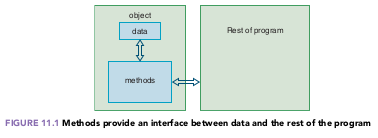
\includegraphics[scale=0.3]{Section_Files/images/Sec04/01.png}
\caption{tex1.}
\end{figure}

{\tiny Web Programming with html5, css, and javascript de John Dean (2019)}
\end{frame}

\begin{frame}{Classes, Constructores, Propiedades, nuevos
Operadores y Metodos}
\justifying



{\tiny Web Programming with html5, css, and javascript de John Dean (2019)}
\end{frame}

\begin{frame}{Generalidades de la POO}
\justifying



{\tiny Web Programming with html5, css, and javascript de John Dean (2019)}
\end{frame}

\begin{frame}{Generalidades de la POO}
\justifying



{\tiny Web Programming with html5, css, and javascript de John Dean (2019)}
\end{frame}

\begin{frame}{Generalidades de la POO}
\justifying



{\tiny Web Programming with html5, css, and javascript de John Dean (2019)}
\end{frame}